\subsection{Dataset Abstractions}
Visualization tools often decompose data into structure and
attributes~\cite{vtk}. Due to the discrete nature of digital
computers, any continuous function to be estimated must be sampled and
measured at a discrete set of points. However, rendering a
visualization typically requires knowledge of the values between the
samples to produce a perceptually continuous images from arbitrary
viewpoints. Structure encapsulates both the locations and connectivity
relations onto which attributes are superimposed where connectivity
serves to constrain the interpolation problem. Note that some authors
further decompose structure further into topology and
geometry~\cite{weiler}, however, in the context of this research,
topology is synonymous with the structure
abstraction. Figure~\ref{fig:data_hierarchy} outlines the data model
abstraction adopted by \sciwms{}. A dataset is composed of attributes
and an associated structure, further classified as a regular or
irregular topology, known as \cgrid{} and \ugrid{} topologies in
\sciwms{} documentation.

\begin{figure}[ht!]
  \centering
  \begin{subfigure}[t]{0.45\textwidth}
    \includegraphics[width=\textwidth]{../figs/data_model_hierarchy}
  \caption{}
  \label{fig:data_hierarchy}
  \end{subfigure}
  \begin{subfigure}[t]{0.45\textwidth}
    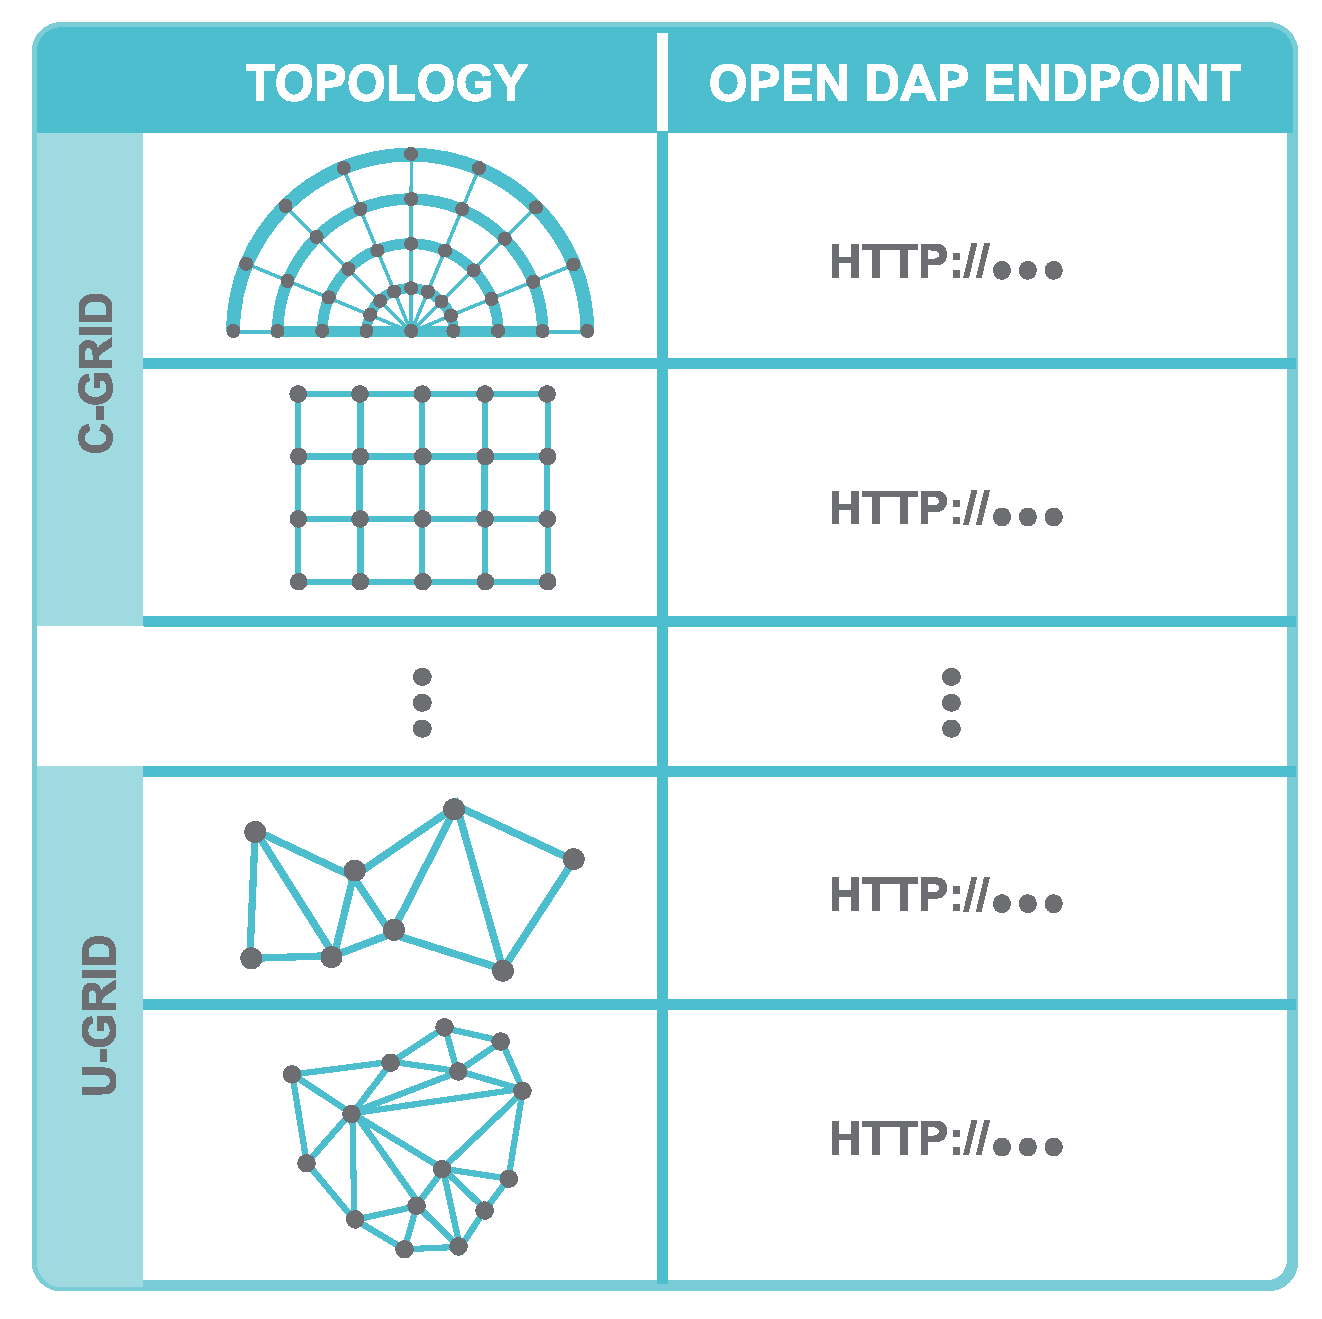
\includegraphics[height=2in]{../figs/sciwms_book_db_topology_endpoint_chart}
    \caption{}
    \label{fig:sciwms_topology_endpoints}
  \end{subfigure}
  \caption{(a) Decomposition hierarchy of the data model. A dataset
    submitted to \sciwms{} is decomposed into attributes and structure
    which is further classified as a regular (\cgrid{}) or irregular
    (\ugrid{}) topologies. (b) \Sciwms{} topology and endpoint data
    store. Topolgies are stored locally in implicit form for \cgrid{}
    or binary R-Tree databases for \ugrid{} topologies. }
\end{figure}
